\section*{CHAPTER 3. OTFS SYSTEM DESIGN AND MODELING}
\addcontentsline{toc}{section}{CHAPTER 3. OTFS SYSTEM DESIGN AND MODELING}

% =========================================================
% Numbering for Chapter 3
% =========================================================
\setcounter{section}{3}
\setcounter{subsection}{0}
\setcounter{subsubsection}{0}
\setcounter{figure}{0}
\setcounter{table}{0}
\setcounter{equation}{0}

\renewcommand{\thefigure}{3.\arabic{figure}}
\renewcommand{\thetable}{3.\arabic{table}}
\renewcommand{\theequation}{3.\arabic{equation}}
\renewcommand{\theHfigure}{3.\arabic{figure}}
\renewcommand{\theHtable}{3.\arabic{table}}
\renewcommand{\theHequation}{3.\arabic{equation}}

% =========================================================
% Chapter Introduction
% =========================================================
This chapter develops the baseline OTFS system used as the reference model for the rest of the thesis. It describes the OTFS transceiver architecture, transmitter and receiver processing chains, delay-Doppler channel model, equivalent input-output relation, and message passing detector, following the main OTFS and iterative detection principles reported in the literature~\cite{Hadani2018OTFS,Raviteja2018OTFSMP,Raviteja2018OTFSInterference}. The objective is to establish a clear baseline before introducing index modulation in Chapter 4.

\begin{figure}[H]
    \centering
    \resizebox{0.98\linewidth}{!}{%
    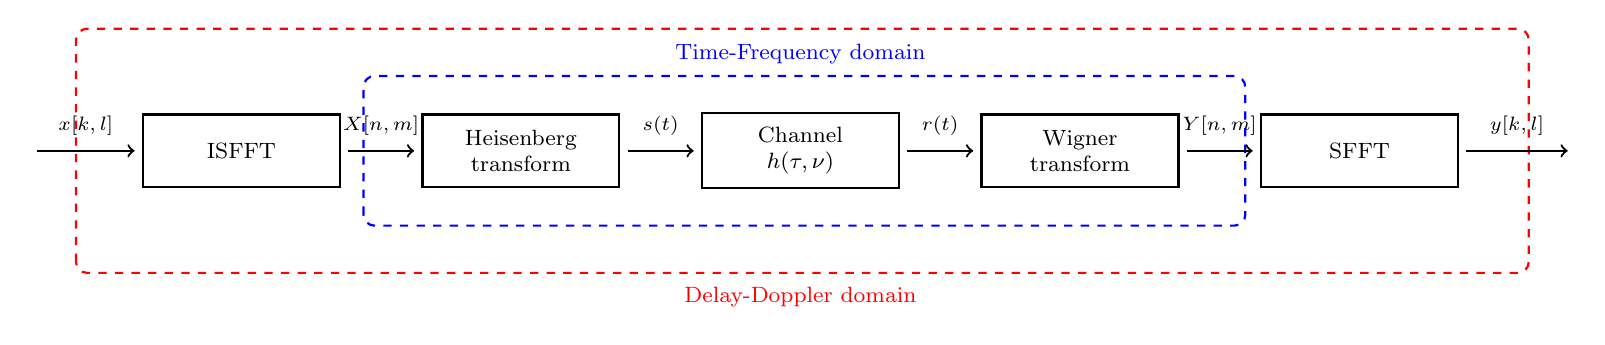
\begin{tikzpicture}[
        block/.style={
            rectangle,
            draw,
            thick,
            align=center,
            text width=2.15cm,
            minimum height=0.92cm,
            font=\footnotesize,
            inner sep=5pt,
            outer sep=0pt
        },
        arrow/.style={
            ->,
            thick,
            shorten >=3pt,
            shorten <=3pt
        }
    ]

        \node[block] (isfft) at (0,0) {ISFFT};
        \node[block] (heis) at (3.55,0) {Heisenberg\\transform};
        \node[block] (chan) at (7.10,0) {Channel\\\(h(\tau,\nu)\)};
        \node[block] (wig) at (10.65,0) {Wigner\\transform};
        \node[block] (sfft) at (14.20,0) {SFFT};

        \draw[dashed, red, thick, rounded corners]
            (-2.10,-1.55) rectangle (16.35,1.55);
        \node[red, font=\footnotesize] at (7.10,-1.86) {Delay-Doppler domain};

        \draw[dashed, blue, thick, rounded corners]
            (1.55,-0.95) rectangle (12.75,0.95);
        \node[blue, font=\footnotesize] at (7.10,1.23) {Time-Frequency domain};

        \draw[arrow] (-2.70,0) -- node[midway, above, yshift=2pt, font=\scriptsize] {\(x[k,l]\)} (isfft.west);
        \draw[arrow] (isfft.east) -- node[midway, above, yshift=2pt, font=\scriptsize] {\(X[n,m]\)} (heis.west);
        \draw[arrow] (heis.east) -- node[midway, above, yshift=2pt, font=\scriptsize] {\(s(t)\)} (chan.west);
        \draw[arrow] (chan.east) -- node[midway, above, yshift=2pt, font=\scriptsize] {\(r(t)\)} (wig.west);
        \draw[arrow] (wig.east) -- node[midway, above, yshift=2pt, font=\scriptsize] {\(Y[n,m]\)} (sfft.west);
        \draw[arrow] (sfft.east) -- node[midway, above, yshift=2pt, font=\scriptsize] {\(y[k,l]\)} (16.95,0);

    \end{tikzpicture}
    }
    \caption{Overall baseline OTFS transceiver architecture}
    \label{fig:baseline_otfs_transceiver_architecture}
\end{figure}


% =========================================================
% Chapter Sections
% =========================================================
\subsection{Design Objectives and System Assumptions}

This section defines the design objectives, system configuration, and main assumptions of the baseline OTFS system used in this thesis. The baseline system is designed as the reference model for the OTFS-IM extension in Chapter 4 and for the numerical comparison in Chapter 5. Therefore, the model must be detailed enough to represent the essential OTFS transmission mechanism, while remaining sufficiently controlled so that the effects of index modulation and pattern selection can be evaluated clearly.

\subsubsection{Design Objectives}

The first objective of the baseline OTFS system is to establish a complete end-to-end transmission chain operating through the delay-Doppler domain. Unlike OFDM, where information symbols are directly arranged in the time-frequency domain, OTFS places data symbols on a two-dimensional delay-Doppler grid before transforming them for transmission. This structure allows the channel effects caused by multipath delay and Doppler shift to be represented more explicitly in the signal model.

The second objective is to provide a fair reference for the OTFS-IM system developed later in this thesis. Since OTFS-IM changes the way information bits are mapped onto the delay-Doppler grid, its performance must be evaluated against a conventional OTFS baseline using the same frame dimensions, modulation order, channel model, noise definition, and detector assumptions. This makes it possible to determine whether the observed performance difference comes from the index-modulation structure and pattern design, rather than from inconsistent simulation settings.

The third objective is to define the receiver structure used as the foundation for later detection analysis. In this thesis, the baseline OTFS receiver uses a message passing detector. This detector is suitable for sparse delay-Doppler channel structures and provides a natural basis for the OTFS-IM receiver, where both QAM symbols and active-position patterns must be detected. Therefore, the baseline OTFS model is not only a comparison curve in the BER results, but also the starting point for the receiver design in the proposed OTFS-IM framework.

\subsubsection{Delay-Doppler Grid and Frame Structure}

The baseline OTFS frame is constructed on a two-dimensional delay-Doppler grid with \(N\) Doppler bins and \(M\) delay bins. The transmitted delay-Doppler symbol matrix is denoted as
\begin{equation}
    \mathbf{x}_{\mathrm{DD}}
    =
    [x[k,l]]
    \in \mathbb{C}^{N \times M},
\end{equation}
where \(k\) is the Doppler index and \(l\) is the delay index. The element \(x[k,l]\) represents the QAM information symbol placed at the \(k\)-th Doppler bin and the \(l\)-th delay bin.

In the baseline OTFS system, all delay-Doppler resource elements are active. Hence, each frame contains
\begin{equation}
    N_{\mathrm{RE}} = MN
\end{equation}
resource elements, and each resource element carries one QAM symbol. This is different from the OTFS-IM system introduced in Chapter 4, where only a subset of positions in each index-modulation block is active and the activation pattern itself also conveys information.

If the QAM modulation order is denoted by \(M_{\mathrm{QAM}}\), then each QAM symbol carries
\begin{equation}
    b_{\mathrm{QAM}} = \log_2(M_{\mathrm{QAM}})
\end{equation}
information bits. Therefore, the total number of information bits transmitted in one baseline OTFS frame is
\begin{equation}
    B_{\mathrm{OTFS}} = MN \log_2(M_{\mathrm{QAM}}).
\end{equation}
The corresponding spectral efficiency, measured in bits per delay-Doppler resource element, is
\begin{equation}
    \eta_{\mathrm{OTFS}}
    =
    \frac{B_{\mathrm{OTFS}}}{MN}
    =
    \log_2(M_{\mathrm{QAM}}).
\end{equation}

For the numerical simulations in this thesis, the baseline OTFS system uses 4-QAM modulation. Thus,
\begin{equation}
    M_{\mathrm{QAM}} = 4,
    \qquad
    b_{\mathrm{QAM}} = 2.
\end{equation}
The baseline spectral efficiency is therefore
\begin{equation}
    \eta_{\mathrm{OTFS}} = 2
    \quad \text{bits/resource element}.
\end{equation}

The selected OTFS grid size is
\begin{equation}
    N = 10, \qquad M = 12,
\end{equation}
which gives
\begin{equation}
    MN = 120
\end{equation}
delay-Doppler resource elements per frame. Since 4-QAM is used, the number of information bits transmitted in one baseline OTFS frame is
\begin{equation}
    B_{\mathrm{OTFS}} = 120 \times 2 = 240
    \quad \text{bits/frame}.
\end{equation}

The main simulation parameters of the baseline OTFS system are summarized in Table~\ref{tab:baseline_otfs_parameters}. This table is placed here because these parameters are repeatedly used in the transmitter design, receiver design, and performance evaluation sections.

\begin{table}[H]
    \centering
    \caption{Baseline OTFS simulation parameters}
    \label{tab:baseline_otfs_parameters}
    \begin{tabular}{c c c}
        \hline
        Parameter & Symbol & Value \\
        \hline
        Number of Doppler bins & \(N\) & 10 \\
        Number of delay bins & \(M\) & 12 \\
        Resource elements per frame & \(MN\) & 120 \\
        QAM modulation order & \(M_{\mathrm{QAM}}\) & 4-QAM \\
        Bits per QAM symbol & \(b_{\mathrm{QAM}}\) & 2 \\
        Baseline spectral efficiency & \(\eta_{\mathrm{OTFS}}\) & 2 bits/resource element \\
        Information bits per OTFS frame & \(B_{\mathrm{OTFS}}\) & 240 bits \\
        \(E_b/N_0\) range & \(E_b/N_0\) & 0:5:20 dB \\
        OTFS Monte Carlo frames & \(N_{\mathrm{fram}}\) & 1000 \\
        OFDM-LMMSE Monte Carlo frames & \(N_{\mathrm{fram,OFDM}}\) & 1000 \\
        \hline
    \end{tabular}
\end{table}

The selected grid size provides a compact simulation setting that keeps the Monte Carlo evaluation computationally feasible. This is important because the thesis later evaluates multiple OTFS-IM configurations and pattern-selection methods under the same channel and noise conditions. The same delay-Doppler frame dimensions are also used as the reference grid for OTFS-IM, so that performance differences can be interpreted in terms of modulation structure and receiver behavior rather than different frame sizes.

\subsubsection{Transceiver Assumptions}

The system considered in this thesis is a single-input single-output transmission system. This assumption keeps the focus on the modulation structure, channel effect, and receiver detection process. Although multi-antenna transmission is important for practical wireless systems, including MIMO processing would introduce additional spatial-domain operations that are outside the main scope of this work.

Perfect timing and frequency synchronization are assumed at the receiver. Under this assumption, the received OTFS frame can be demodulated without additional synchronization errors. This choice is suitable for the baseline design because synchronization impairments would introduce another source of degradation and make it more difficult to isolate the effects of OTFS modulation and OTFS-IM pattern selection.

The receiver is also assumed to have access to the channel parameters required by the detector. In other words, the detection process is evaluated under a perfect-CSI assumption. This does not imply that channel estimation is unimportant in practical OTFS systems. Rather, channel estimation is excluded so that the thesis can focus on modulation, index-pattern design, and detection reliability under controlled conditions.

\subsubsection{Channel Assumptions}

The wireless channel is modeled as a time-varying multipath Rayleigh fading channel in the delay-Doppler domain. Each propagation path is represented by a delay tap, a Doppler tap, and a complex fading coefficient. The delay tap models the propagation delay of a multipath component, while the Doppler tap represents the time variation induced by relative motion or dynamic scattering in the propagation environment.

The complex path coefficients are generated as complex Gaussian random variables with delay-dependent power scaling. As a result, the channel amplitudes follow a Rayleigh fading behavior. Additive white Gaussian noise is then added after the multipath channel. This model allows the simulation to capture the combined effects of multipath fading, delay spread, Doppler spread, and thermal noise.

In this thesis, the Doppler shifts are represented by normalized discrete Doppler taps on the OTFS grid. Therefore, the channel captures Doppler-induced time selectivity without assigning a specific physical velocity in kilometres per hour. This modeling choice is appropriate for the objective of the thesis, which is to evaluate OFDM, OTFS, and OTFS-IM under a common high-Doppler delay-Doppler fading condition, rather than to reproduce a standardized vehicular channel model.

This assumption should be interpreted carefully. The simulated channel represents the main impairment associated with high-mobility communication, namely Doppler-induced time variation. However, it is not claimed to correspond exactly to a particular vehicle speed. For this reason, the channel is described as a high-Doppler or mobility-like delay-Doppler fading channel in the simulation discussion.

\subsubsection{Fairness Criteria for Comparison}

A key requirement of the simulation framework is fairness. The OFDM, OTFS, and OTFS-IM systems are evaluated over the same \(E_b/N_0\) range and under the same channel generation mechanism. This ensures that the performance differences observed in Chapter 5 mainly arise from the modulation and detection structures, rather than from inconsistent channel or noise assumptions.

The OFDM reference used in this thesis is denoted as OFDM-LMMSE. It uses a full-frame linear minimum mean square error equalizer with channel knowledge. This makes the OFDM baseline stronger and more meaningful than a simple one-tap OFDM receiver in a time-varying channel. Therefore, any gain achieved by OTFS or OTFS-IM is compared against an OFDM receiver that already includes explicit equalization.

For the OTFS baseline, the same channel realization style and noise definition are used. The receiver uses a message passing detector, which is suitable for sparse delay-Doppler channel structures. In Chapter 4, the OTFS-IM receiver builds on this detection framework by using probability information to identify both QAM symbols and activation patterns.

Spectral efficiency is also considered when interpreting the results. Since the baseline OTFS system with 4-QAM has a spectral efficiency of \(2\) bits/resource element, OTFS-IM configurations with the same value are treated as rate-fair comparisons. Configurations with lower spectral efficiency are interpreted as reliability-oriented cases, where reduced rate is exchanged for improved BER performance. This distinction is important because OTFS-IM does not automatically outperform OTFS in every configuration; its advantage depends on the trade-off among spectral efficiency, pattern detection reliability, and symbol detection accuracy.

\subsubsection{Scope of the Baseline Model}

The baseline OTFS model is intentionally compact and controlled. It does not include channel coding, channel estimation error, synchronization offset, MIMO transmission, or standardized 5G channel profiles. These components are important in practical systems, but including all of them would make it harder to isolate the contribution of OTFS-IM activation-pattern design.

The role of the baseline model is therefore to provide a clean and consistent reference system. It defines the delay-Doppler frame, the modulation format, the channel assumptions, and the receiver detection structure used throughout the thesis. Based on this baseline, Chapter 4 introduces index modulation into the OTFS grid and studies how activation-pattern design affects index BER, symbol BER, pattern error rate, and total BER.

\subsection{OTFS Transmitter Design}

\subsubsection{Overview of the Transmitter Processing Chain}

The OTFS transmitter is designed to convert a binary information sequence into a time-domain waveform suitable for transmission over a time-varying multipath channel. The key idea is that the information symbols are first arranged in the delay-Doppler domain, rather than being transmitted directly in the time-frequency domain. This processing structure allows the transmitted frame to be associated with the delay and Doppler characteristics of the wireless channel.

The overall transmitter chain used in the baseline OTFS system is illustrated in Fig.~\ref{fig:otfs_transmitter_chain}. The input bit sequence is first mapped into QAM symbols. These symbols are then placed on the delay-Doppler grid to form the matrix \(\mathbf{x}_{\mathrm{DD}}\). After that, the inverse symplectic finite Fourier transform is applied to convert the delay-Doppler symbols into the time-frequency domain. The resulting time-frequency symbols are finally transformed into a time-domain transmit signal by the Heisenberg transform, or equivalently by its discrete implementation in the simulation.

\begin{figure}[H]
    \centering
    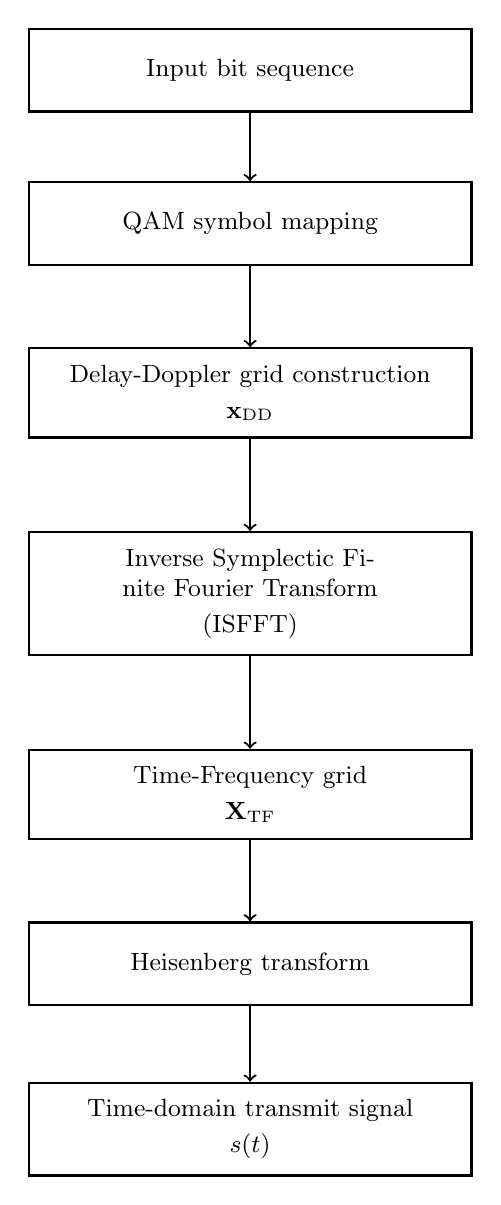
\begin{tikzpicture}[
        block/.style={
            rectangle,
            draw,
            thick,
            align=center,
            text width=5.2cm,
            minimum height=1.05cm,
            font=\small,
            inner sep=6pt
        },
        arrow/.style={
            ->,
            thick,
            shorten >=0pt,
            shorten <=0pt
        }
    ]

        \node[block] (bits) at (0,0) {Input bit sequence};
        \node[block] (qam) at (0,-1.95) {QAM symbol mapping};
        \node[block] (dd) at (0,-4.10) {Delay-Doppler grid construction\\[2pt]\(\mathbf{x}_{\mathrm{DD}}\)};
        \node[block] (isfft) at (0,-6.65) {Inverse Symplectic Finite Fourier Transform\\[2pt](ISFFT)};
        \node[block] (tf) at (0,-9.20) {Time-Frequency grid\\[2pt]\(\mathbf{X}_{\mathrm{TF}}\)};
        \node[block] (heis) at (0,-11.35) {Heisenberg transform};
        \node[block] (tx) at (0,-13.45) {Time-domain transmit signal\\[2pt]\(s(t)\)};

        \draw[arrow] (bits.south) -- (qam.north);
        \draw[arrow] (qam.south) -- (dd.north);
        \draw[arrow] (dd.south) -- (isfft.north);
        \draw[arrow] (isfft.south) -- (tf.north);
        \draw[arrow] (tf.south) -- (heis.north);
        \draw[arrow] (heis.south) -- (tx.north);

    \end{tikzpicture}
    \caption{Baseline OTFS transmitter processing chain}
    \label{fig:otfs_transmitter_chain}
\end{figure}

The transmitter can therefore be viewed as a sequence of four main operations. The first operation is bit-to-symbol mapping, where the input bits are grouped and mapped to QAM constellation points. The second operation is delay-Doppler grid construction, where the QAM symbols are arranged over the \(N \times M\) OTFS frame. The third operation is the inverse symplectic finite Fourier transform, which maps the delay-Doppler representation to the time-frequency representation. The final operation is time-domain signal generation, where the time-frequency samples are converted into the transmitted waveform.

This separation of operations is useful because each stage has a distinct role in the OTFS system. The QAM mapper determines the number of bits carried by each active resource element. The delay-Doppler grid defines the information-bearing structure of the OTFS frame. The ISFFT performs the domain transformation required by OTFS modulation, while the Heisenberg transform generates the signal that is actually transmitted through the channel. In the baseline OTFS system, all delay-Doppler grid positions are active, which makes the transmitter structure simpler than the OTFS-IM transmitter introduced in Chapter 4.

In the discrete simulation model, the transmitter follows the same conceptual chain. A random bit sequence is generated and mapped to 4-QAM symbols. The symbol vector is reshaped into an \(N \times M\) delay-Doppler matrix. The OTFS modulation stage then performs the discrete transform operations and serializes the result into a time-domain vector. This vector is used as the input to the multipath delay-Doppler channel model described in the next section.

\subsubsection{Bit-to-QAM Symbol Mapping}

The first stage of the baseline OTFS transmitter is the mapping of information bits to QAM symbols. In the OTFS notation used in this thesis, the information symbols before modulation are denoted by \(x[k,l]\), where \(k\) is the Doppler index and \(l\) is the delay index. These symbols form the delay-Doppler information grid that will later be transformed into the time-frequency domain.

For one OTFS frame, the transmitter generates a binary information sequence with
\begin{equation}
    B_{\mathrm{OTFS}} = MN\log_2(M_{\mathrm{QAM}})
\end{equation}
bits, where \(M_{\mathrm{QAM}}\) is the QAM modulation order. For the baseline setup, \(N=10\), \(M=12\), and \(M_{\mathrm{QAM}}=4\), so one OTFS frame contains
\begin{equation}
    B_{\mathrm{OTFS}} = 10 \times 12 \times \log_2(4) = 240
\end{equation}
information bits.

The input bit sequence is divided into groups of \(\log_2(M_{\mathrm{QAM}})\) bits. Each group is converted into a decimal symbol index and then mapped to one QAM constellation point. This produces a vector of \(MN\) complex-valued QAM symbols. This mapping is represented by
\begin{equation}
    \mathbf{x}
    =
    \mathcal{Q}_{M_{\mathrm{QAM}}}
    \left(
    \mathbf{b}
    \right),
\end{equation}
where \(\mathcal{Q}_{M_{\mathrm{QAM}}}(\cdot)\) denotes grouping the input bits and mapping each group to an \(M_{\mathrm{QAM}}\)-ary QAM constellation point.

After QAM mapping, the symbol vector is reshaped into the delay-Doppler grid as
\begin{equation}
    \mathbf{x}_{\mathrm{DD}}
    =
    \left[
    x[k,l]
    \right]_{N \times M}.
\end{equation}
In the code, this step is performed by
\begin{equation}
    \mathbf{x}_{\mathrm{DD}}
    =
    \mathrm{reshape}(\mathbf{x},N,M).
\end{equation}

For the baseline OTFS system, all positions on the delay-Doppler grid are active. Therefore, every element \(x[k,l]\) carries one QAM symbol. This is an important difference from the OTFS-IM transmitter introduced in Chapter 4, where only selected positions are active and the active-position pattern itself also conveys information.

With 4-QAM modulation, each delay-Doppler resource element carries two information bits. Therefore, the baseline OTFS transmitter maps the 240 input bits of one frame into 120 QAM symbols and places them over the full \(10 \times 12\) delay-Doppler grid. The resulting matrix \(\mathbf{x}_{\mathrm{DD}}\) is then used as the input to the OTFS modulation block.

\subsubsection{Delay-Doppler Grid Construction}

After QAM symbol mapping, the next stage is to arrange the modulated symbols onto the OTFS delay-Doppler grid. This grid is the information-bearing domain of OTFS. Instead of assigning symbols directly to time-frequency resource elements as in OFDM, OTFS first places the QAM symbols in the delay-Doppler domain. The subsequent OTFS modulation stages then spread these symbols over the time-frequency plane before transmission.

Let the QAM symbol vector generated by the previous stage be denoted by
\begin{equation}
    \mathbf{x}
    =
    [x_0,x_1,\ldots,x_{MN-1}]^T.
\end{equation}
This vector contains \(MN\) complex-valued QAM symbols. In the baseline OTFS transmitter, these symbols are reshaped into the delay-Doppler symbol matrix
\begin{equation}
    \mathbf{x}_{\mathrm{DD}}
    =
    [x[k,l]]
    \in \mathbb{C}^{N \times M},
\end{equation}
where \(k=0,1,\ldots,N-1\) denotes the Doppler index and \(l=0,1,\ldots,M-1\) denotes the delay index.

The mapping from the one-dimensional QAM symbol vector to the two-dimensional delay-Doppler grid can be written as
\begin{equation}
    x[k,l] = x_{k + lN},
    \qquad
    0 \leq k \leq N-1,\quad 0 \leq l \leq M-1.
\end{equation}
This indexing follows a fixed column-wise ordering when the one-dimensional symbol sequence is arranged into the \(N \times M\) delay-Doppler grid. Equivalently, the reshaping operation can be represented as
\begin{equation}
    \mathbf{x}_{\mathrm{DD}}
    =
    \mathrm{reshape}(\mathbf{x},N,M).
\end{equation}

For the baseline OTFS system, every position of the delay-Doppler grid is occupied by one QAM symbol. Therefore, the grid contains no inactive resource elements. This full-grid structure is important because it defines the conventional OTFS reference system. In Chapter 4, the OTFS-IM transmitter modifies this structure by dividing the grid into index-modulation blocks and activating only selected positions inside each block.

For the simulation configuration used in this thesis, the grid size is \(N=10\) and \(M=12\). Hence, the delay-Doppler grid contains \(120\) symbol positions. With 4-QAM modulation, the transmitter maps \(240\) input bits into \(120\) QAM symbols and places them over the full delay-Doppler grid. The resulting matrix \(\mathbf{x}_{\mathrm{DD}}\) is then used as the input to the inverse symplectic finite Fourier transform in the next stage of the OTFS modulator.

A conceptual view of the baseline delay-Doppler grid is shown in Fig.~\ref{fig:baseline_dd_grid}. Each cell represents one delay-Doppler resource element, and all cells are active in the baseline OTFS system.

\begin{figure}[H]
    \centering
    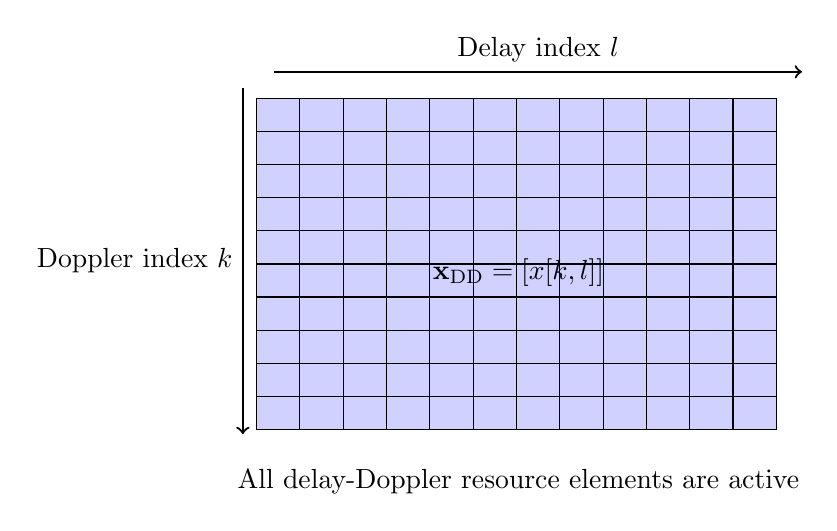
\begin{tikzpicture}[
        cell/.style={
            rectangle,
            draw,
            minimum width=0.55cm,
            minimum height=0.42cm
        },
        active/.style={
            fill=blue!18
        }
    ]

        \foreach \i in {0,...,9} {
            \foreach \j in {0,...,11} {
                \node[cell, active] at (\j*0.55,-\i*0.42) {};
            }
        }

        \draw[->, thick] (-0.45,0.35) -- (-0.45,-4.05)
            node[midway, left] {Doppler index \(k\)};
        \draw[->, thick] (-0.05,0.55) -- (6.65,0.55)
            node[midway, above] {Delay index \(l\)};

        \node at (3.05,-2.0) {\(\mathbf{x}_{\mathrm{DD}}=[x[k,l]]\)};
        \node[align=center] at (3.05,-4.65) {All delay-Doppler resource elements are active};

    \end{tikzpicture}
    \caption{Baseline OTFS delay-Doppler grid with full resource activation}
    \label{fig:baseline_dd_grid}
\end{figure}

\subsubsection{Inverse Symplectic Finite Fourier Transform}

After the QAM symbols are arranged on the delay-Doppler grid, the next step of the OTFS transmitter is to transform them into the time-frequency domain. This operation is performed by the inverse symplectic finite Fourier transform. The ISFFT is one of the core operations of OTFS modulation because it connects the information-bearing delay-Doppler representation to the time-frequency representation used for waveform generation.

Let the delay-Doppler symbol matrix be denoted by
\begin{equation}
    \mathbf{x}_{\mathrm{DD}} = [x[k,l]],
\end{equation}
where \(k=0,1,\ldots,N-1\) is the Doppler index and \(l=0,1,\ldots,M-1\) is the delay index. The ISFFT maps \(x[k,l]\) into the time-frequency symbols \(X[n,m]\), where \(n=0,1,\ldots,N-1\) denotes the time index and \(m=0,1,\ldots,M-1\) denotes the frequency index.

Using the OTFS convention adopted in this thesis, the ISFFT can be written as
\begin{equation}
    X[n,m]
    =
    \frac{1}{\sqrt{MN}}
    \sum_{k=0}^{N-1}
    \sum_{l=0}^{M-1}
    x[k,l]
    e^{j2\pi\left(\frac{nk}{N}-\frac{ml}{M}\right)}.
    \label{eq:isfft}
\end{equation}
The resulting matrix
\begin{equation}
    \mathbf{X}_{\mathrm{TF}}
    =
    [X[n,m]]
    \in \mathbb{C}^{N \times M}
\end{equation}
represents the OTFS frame in the time-frequency domain.

The structure of the ISFFT is different from a conventional two-dimensional inverse Fourier transform because the signs of the Fourier kernels are opposite along the two dimensions. This symplectic structure reflects the dual relationship between the delay-Doppler and time-frequency domains. In particular, the Doppler dimension is transformed with respect to the time index, while the delay dimension is transformed with respect to the frequency index.

For the discrete implementation used in the simulation model, the ISFFT operation is evaluated through a pair of finite Fourier transforms along the two grid dimensions:
\begin{equation}
    \mathbf{X}_{\mathrm{TF}}
    =
    \mathrm{fft}
    \left(
    \mathrm{ifft}
    \left(
    \mathbf{x}_{\mathrm{DD}}
    \right)^T
    \right)^T
    \bigg/
    \sqrt{\frac{M}{N}}.
    \label{eq:isfft_matlab}
\end{equation}
This expression is the matrix-form counterpart of the ISFFT in \eqref{eq:isfft}. The two transform directions correspond to the delay and Doppler dimensions, while the normalization factor preserves the energy scale of the OTFS frame.

The normalization factor is included to preserve the signal energy across the domain transformation. This is important for BER simulation because the noise variance is computed from the selected \(E_b/N_0\) value. If the transform scaling were inconsistent, the effective received SNR would be shifted, making the BER comparison between OFDM, OTFS, and OTFS-IM unfair.

After the ISFFT, each delay-Doppler information symbol has been spread across the time-frequency grid. This spreading property is one of the reasons OTFS is suitable for time-varying multipath channels. Instead of assigning each information symbol to a single time-frequency resource element, OTFS distributes the symbol over the frame before waveform generation. The time-frequency matrix \(\mathbf{X}_{\mathrm{TF}}\) is then passed to the Heisenberg transform to generate the time-domain transmit signal.

\subsubsection{Heisenberg Transform and Time-Domain Signal Generation}

After the ISFFT, the OTFS frame is represented by the time-frequency symbol matrix
\begin{equation}
    \mathbf{X}_{\mathrm{TF}} = [X[n,m]],
\end{equation}
where \(n=0,1,\ldots,N-1\) is the time index and \(m=0,1,\ldots,M-1\) is the frequency index. The purpose of the Heisenberg transform is to convert these time-frequency samples into a continuous-time transmit waveform.

In the general OTFS formulation, the transmitted signal can be expressed as
\begin{equation}
    s(t)
    =
    \sum_{n=0}^{N-1}
    \sum_{m=0}^{M-1}
    X[n,m]\,
    g_{\mathrm{tx}}(t-nT)
    e^{j2\pi m\Delta f(t-nT)},
    \label{eq:heisenberg_transform}
\end{equation}
where \(g_{\mathrm{tx}}(t)\) is the transmit pulse, \(T\) is the symbol duration, and \(\Delta f\) is the subcarrier spacing. This expression shows that each time-frequency sample \(X[n,m]\) modulates a time-shifted and frequency-shifted version of the transmit pulse.

The Heisenberg transform can be viewed as the waveform-generation stage of the OTFS transmitter. While the delay-Doppler grid defines where the information symbols are placed, and the ISFFT maps them into the time-frequency domain, the Heisenberg transform produces the actual signal that enters the wireless channel. Therefore, it plays a role similar to the multicarrier modulation stage in OFDM, but it operates on the time-frequency samples generated from the delay-Doppler information grid.

In the discrete model used in this thesis, the Heisenberg transform is represented after the ISFFT by applying an inverse Fourier transform along the frequency-related dimension:
\begin{equation}
    \mathbf{s}_{\mathrm{mat}}
    =
    \mathrm{ifft}
    \left(
    \mathbf{X}_{\mathrm{TF}}^T
    \right)
    \sqrt{M}.
    \label{eq:heisenberg_matlab}
\end{equation}
This matrix \(\mathbf{s}_{\mathrm{mat}}\) contains the time-domain samples associated with the time-frequency grid \(\mathbf{X}_{\mathrm{TF}}\). The scaling factor keeps the discrete waveform normalization consistent with the ISFFT stage.

The matrix \(\mathbf{s}_{\mathrm{mat}}\) contains the discrete time-domain samples before serialization. To form the transmit vector, the matrix is converted into a column vector according to
\begin{equation}
    \mathbf{s}
    =
    \mathrm{vec}
    \left(
    \mathbf{s}_{\mathrm{mat}}
    \right).
    \label{eq:tx_vector}
\end{equation}
The vectorization step preserves the sample ordering used by the OTFS frame and produces a one-dimensional transmit sequence suitable for the channel model.

The output vector \(\mathbf{s}\) is the discrete-time transmit signal used as the input to the wireless channel model. In the simulation framework, this signal is passed to the time-varying multipath channel model, where delay taps, Doppler taps, fading coefficients, and additive noise are applied. Therefore, the Heisenberg transform and serialization stage completes the baseline OTFS transmitter processing chain.

\subsubsection{Discrete Processing Summary}

The baseline OTFS transmitter can be summarized by three discrete signal-processing operations: ISFFT, discrete Heisenberg transformation, and serialization. The input is the delay-Doppler matrix \(\mathbf{x}_{\mathrm{DD}}\), obtained by arranging the QAM symbol vector according to the \(N \times M\) frame ordering described earlier. The output is the time-domain transmit vector \(\mathbf{s}\).

The complete discrete transmitter chain can therefore be summarized as
\begin{equation}
\begin{aligned}
    \mathbf{X}_{\mathrm{TF}}
    &=
    \mathrm{fft}
    \left(
    \mathrm{ifft}
    \left(
    \mathbf{x}_{\mathrm{DD}}
    \right)^T
    \right)^T
    \bigg/
    \sqrt{\frac{M}{N}},
    \\
    \mathbf{s}_{\mathrm{mat}}
    &=
    \mathrm{ifft}
    \left(
    \mathbf{X}_{\mathrm{TF}}^T
    \right)
    \sqrt{M},
    \\
    \mathbf{s}
    &=
    \mathrm{vec}
    \left(
    \mathbf{s}_{\mathrm{mat}}
    \right).
\end{aligned}
\end{equation}

This compact representation is important for the rest of the thesis because the same OTFS modulation principle is used for both the baseline OTFS system and the later OTFS-IM system. The difference between the two systems is not in the modulation transform itself, but in the construction of the delay-Doppler input matrix. In the baseline OTFS system, every delay-Doppler position carries a QAM symbol, while in OTFS-IM only selected positions are active according to an index-modulation pattern.

\subsubsection{Summary of the Baseline OTFS Transmitter}

The baseline OTFS transmitter converts a binary information sequence into a time-domain signal through a sequence of delay-Doppler and time-frequency processing stages. The input bits are first mapped to QAM symbols and arranged on the delay-Doppler grid as \(x[k,l]\). In the baseline system, all delay-Doppler resource elements are active, so every grid position carries one QAM symbol.

The delay-Doppler symbol matrix \(\mathbf{x}_{\mathrm{DD}}\) is then transformed into the time-frequency domain by the ISFFT. This produces the time-frequency matrix \(\mathbf{X}_{\mathrm{TF}}\), whose elements \(X[n,m]\) are used for waveform generation. The discrete Heisenberg transform is finally applied to obtain the time-domain transmit vector \(\mathbf{s}\).

The transmitter chain can be summarized as
\begin{equation}
    \mathbf{b}
    \rightarrow
    \mathbf{x}
    \rightarrow
    \mathbf{x}_{\mathrm{DD}}
    \xrightarrow{\mathrm{ISFFT}}
    \mathbf{X}_{\mathrm{TF}}
    \xrightarrow{\mathrm{Heisenberg}}
    \mathbf{s}.
\end{equation}

This structure highlights the main difference between OTFS and conventional OFDM. In OFDM, information symbols are directly assigned to time-frequency resource elements. In OTFS, the information symbols are first placed in the delay-Doppler domain and then spread across the time-frequency plane before transmission. This spreading allows the transmitted frame to interact with the delay-Doppler structure of the wireless channel.

The same OTFS modulation block is reused later for the OTFS-IM transmitter. The key difference is the construction of the delay-Doppler input matrix. In the baseline OTFS system, every grid position is active. In OTFS-IM, only selected positions are active, and their indices carry additional information bits. Therefore, the baseline transmitter developed in this section provides the foundation for the OTFS-IM design in Chapter 4.

After the time-domain signal \(\mathbf{s}\) is generated, it is passed through the time-varying multipath channel. The design of this channel model and its delay-Doppler characteristics are discussed in the next section.


\subsection{Channel Model Design}

This section describes the wireless channel model used in the baseline OTFS simulation. The purpose of the channel model is to represent a time-varying multipath propagation environment with both delay and Doppler effects. The same channel generation mechanism is used for OFDM-LMMSE, baseline OTFS, and OTFS-IM so that the performance comparison in Chapter 5 remains consistent.

\subsubsection{Time-Varying Multipath Channel Overview}

In OTFS theory, a time-varying wireless channel can be represented in the delay-Doppler domain by a finite number of propagation paths. Each path is characterized by a delay, a Doppler shift, and a complex channel coefficient. This representation is suitable for OTFS because the transmitted information symbols are first arranged in the delay-Doppler domain before being transformed for transmission.

In the simulation model used in this thesis, the continuous delay-Doppler channel is represented by discrete channel taps. The channel is described by
\begin{equation}
    \{h_i,l_i,\nu_i\}_{i=1}^{P},
\end{equation}
where \(P\) is the number of channel paths, \(h_i\) is the complex fading coefficient of the \(i\)-th path, \(l_i\) is the discrete delay tap, and \(\nu_i\) is the discrete Doppler tap. In this model, \(\nu_i\) denotes a Doppler-tap index on the OTFS grid rather than a physical Doppler frequency in hertz. The Doppler tap is therefore represented as a normalized integer index on the OTFS Doppler grid.

A conceptual representation of the channel model is shown in Fig.~\ref{fig:discrete_multipath_channel}. The transmitted signal is passed through several delayed, Doppler-shifted, and faded propagation paths. The path contributions are then summed and complex additive white Gaussian noise is added.

\begin{figure}[H]
    \centering
    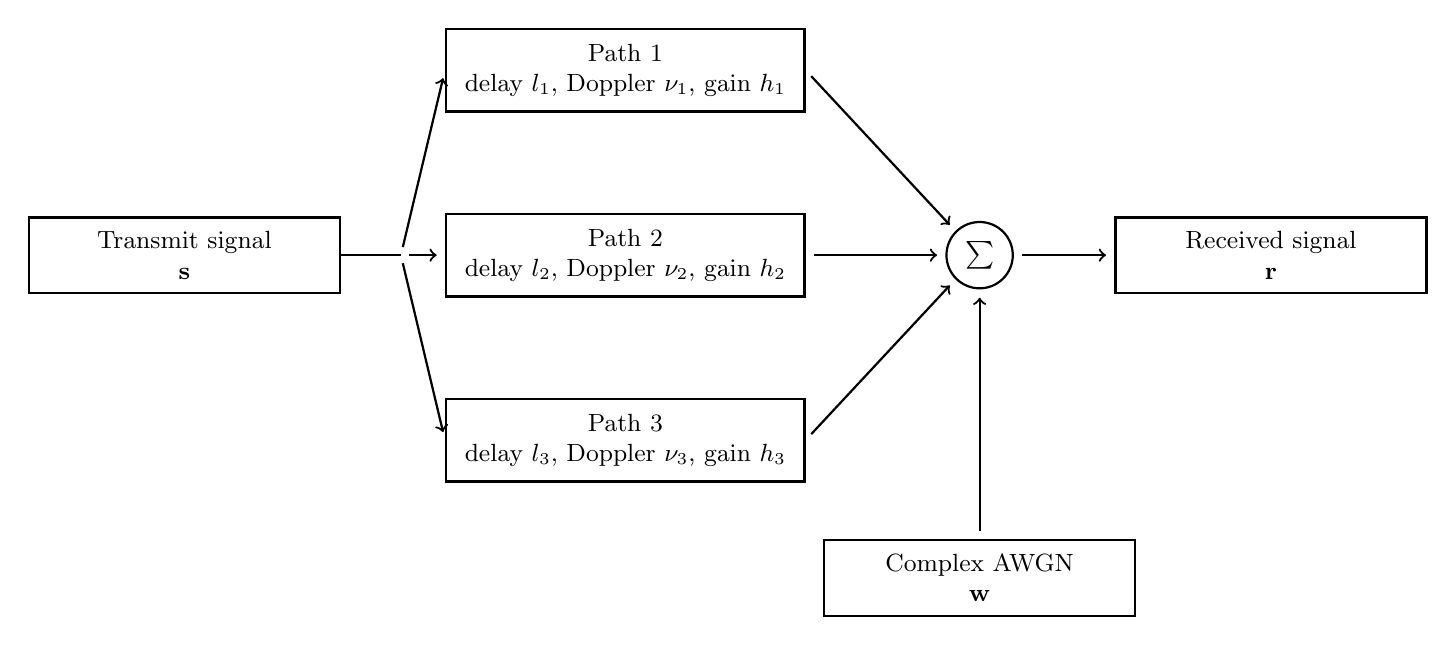
\begin{tikzpicture}[
        block/.style={
            rectangle,
            draw,
            thick,
            align=center,
            text width=3.6cm,
            minimum height=0.9cm,
            font=\small,
            inner sep=5pt
        },
        pathblock/.style={
            rectangle,
            draw,
            thick,
            align=center,
            text width=4.2cm,
            minimum height=1.05cm,
            font=\small,
            inner sep=5pt
        },
        sum/.style={
            circle,
            draw,
            thick,
            minimum size=0.8cm,
            font=\small
        },
        arrow/.style={
            ->,
            thick,
            shorten >=3pt,
            shorten <=3pt
        }
    ]

        \node[block] (input) at (0,0) {Transmit signal\\\(\mathbf{s}\)};

        \coordinate (split) at (2.75,0);

        \node[pathblock] (p1) at (5.6,2.35) {Path 1\\delay \(l_1\), Doppler \(\nu_1\), gain \(h_1\)};
        \node[pathblock] (p2) at (5.6,0) {Path 2\\delay \(l_2\), Doppler \(\nu_2\), gain \(h_2\)};
        \node[pathblock] (p3) at (5.6,-2.35) {Path 3\\delay \(l_3\), Doppler \(\nu_3\), gain \(h_3\)};

        \node[sum] (sum) at (10.1,0) {\(\sum\)};
        \node[block] (noise) at (10.1,-4.1) {Complex AWGN\\\(\mathbf{w}\)};
        \node[block] (output) at (13.8,0) {Received signal\\\(\mathbf{r}\)};

        \draw[thick] (input.east) -- (split);
        \draw[arrow] (split) -- (p1.west);
        \draw[arrow] (split) -- (p2.west);
        \draw[arrow] (split) -- (p3.west);

        \draw[arrow] (p1.east) -- (sum.north west);
        \draw[arrow] (p2.east) -- (sum.west);
        \draw[arrow] (p3.east) -- (sum.south west);

        \draw[arrow] (noise.north) -- (sum.south);
        \draw[arrow] (sum.east) -- (output.west);

    \end{tikzpicture}
    \caption{Discrete time-varying multipath channel model}
    \label{fig:discrete_multipath_channel}
\end{figure}

\subsubsection{Delay and Doppler Tap Representation}

The channel model uses three multipath components, so
\begin{equation}
    P = 3.
\end{equation}
The delay taps are fixed as
\begin{equation}
    \mathbf{l} = [0,1,2],
\end{equation}
which means that the three paths arrive with different discrete delays. These delay taps create delay spread in the received signal.

The Doppler taps are generated randomly for each channel realization. Each Doppler tap belongs to the set
\begin{equation}
    \nu_i \in \{-4,-3,-2,-1,0,1,2,3,4,5\}.
\end{equation}

The Doppler taps introduce time variation through phase rotation across the transmitted samples. A larger absolute Doppler tap produces faster phase variation. Since the Doppler values are represented as discrete indices, the model captures Doppler-induced time selectivity without assigning a specific physical velocity in kilometres per hour.

\subsubsection{Rayleigh Fading Path Coefficients}

Each channel path is assigned a complex fading coefficient. The channel coefficients are modeled as
\begin{equation}
    h_i
    =
    \sqrt{\frac{e^{-l_i}}{2}}
    \left(
    a_i + jb_i
    \right),
    \label{eq:channel_coeff}
\end{equation}
where \(a_i\) and \(b_i\) are independent real Gaussian random variables.

Because \(h_i\) is complex Gaussian, its amplitude follows a Rayleigh fading behavior. The factor \(e^{-l_i}\) introduces a delay-dependent power profile, where paths with larger delays have lower average power. This produces a simple exponentially decaying multipath channel profile.

\subsubsection{Discrete Channel Input-Output Operation}

Let \(\mathbf{s}\) be the transmitted time-domain vector generated by the OTFS transmitter. The channel output is obtained by summing the contribution of all delayed and Doppler-shifted paths. A compact discrete representation is
\begin{equation}
    r[q]
    =
    \sum_{i=1}^{P}
    h_i
    e^{j\phi_i(q)}
    s[q-l_i]
    +
    w[q],
    \label{eq:discrete_channel}
\end{equation}
where \(q\) is the discrete time-sample index, \(l_i\) is the delay tap, \(e^{j\phi_i(q)}\) is the Doppler-induced phase rotation, and \(w[q]\) is the additive noise sample.

The Doppler phase rotation is represented through the exponential term
\begin{equation}
    \exp
    \left(
    j\frac{2\pi}{M}
    q
    \frac{\nu_i}{N}
    \right).
\end{equation}
Each path contribution is then circularly shifted according to its delay tap and weighted by its complex channel coefficient.

Before applying the channel, a cyclic-prefix-like extension is added using the maximum delay tap. After the channel and noise are applied, this prefix part is removed so that the received vector has the same length as the transmitted OTFS frame.

\subsubsection{Additive White Gaussian Noise}

After the multipath channel output is generated, complex additive white Gaussian noise is added. The noise sample is modeled as
\begin{equation}
    w[q]
    =
    \sqrt{\frac{\sigma^2}{2}}
    \left(
    n_{\mathrm{I}}[q] + jn_{\mathrm{Q}}[q]
    \right),
    \label{eq:awgn}
\end{equation}
where \(n_{\mathrm{I}}[q]\) and \(n_{\mathrm{Q}}[q]\) are independent real Gaussian random variables with zero mean and unit variance.

The noise variance \(\sigma^2\) is computed from the selected \(E_b/N_0\) value and the spectral efficiency of the corresponding transmission scheme. Therefore, OFDM-LMMSE, OTFS, and OTFS-IM are evaluated under consistent energy-per-bit conditions.

\subsubsection{Channel Parameters Used in Simulation}

The main channel parameters are summarized in Table~\ref{tab:channel_model_parameters}. These parameters are used consistently across the baseline OTFS system, the OFDM-LMMSE reference, and the OTFS-IM simulations.

\begin{table}[H]
    \centering
    \caption{Delay-Doppler channel parameters used in simulation}
    \label{tab:channel_model_parameters}
    \begin{tabular}{c c c}
        \hline
        Parameter & Symbol & Value \\
        \hline
        Number of channel paths & \(P\) & 3 \\
        Delay taps & \(\mathbf{l}\) & \([0,1,2]\) \\
        Doppler tap range & \(\nu_i\) & \(-4\) to \(5\) \\
        Fading coefficient & \(h_i\) & Complex Gaussian \\
        Fading amplitude & \(|h_i|\) & Rayleigh-type fading \\
        Delay power profile & -- & Exponential decay \(e^{-l_i}\) \\
        Noise model & \(w[q]\) & Complex AWGN \\
        CSI assumption & -- & Known channel parameters at receiver \\
        \hline
    \end{tabular}
\end{table}

\subsubsection{Channel Model Summary}

The channel model used in this thesis is a discrete delay-Doppler multipath Rayleigh fading channel with additive white Gaussian noise. It includes three propagation paths, fixed delay taps, random discrete Doppler taps, and complex Gaussian fading coefficients. This structure is consistent with the OTFS principle that channels with delay and Doppler dispersion can be represented compactly in the delay-Doppler domain.

The model is intentionally controlled rather than fully standardized. It does not assign a specific mobile velocity or use a complete 3GPP channel profile. Instead, it provides a common high-Doppler delay-Doppler fading environment for comparing OFDM-LMMSE, OTFS, and OTFS-IM under the same channel conditions.


\subsection{OTFS Receiver Design}

The receiver of the baseline OTFS system performs the inverse operation of the transmitter front-end. After the transmitted waveform passes through the time-varying multipath channel, the received time-domain signal is first converted back to the time-frequency domain and then transformed to the delay-Doppler domain. The resulting delay-Doppler symbols are not directly used for hard symbol decisions. Instead, they form the observation vector for the message passing detector described in Section 3.6.

In the simulation model, the receiver processing contains two main operations: the Wigner transform and the symplectic finite Fourier transform (SFFT). The Wigner transform converts the received time-domain samples into a time-frequency grid, while the SFFT converts the time-frequency grid back to the delay-Doppler domain.

\subsubsection{Overview of the Receiver Processing Chain}

The receiver starts from the sampled received signal \(\mathbf{r}\), which includes the effect of the doubly dispersive channel and additive noise. This signal is reshaped into a two-dimensional matrix so that the receiver can process it over the same \(M \times N\) OTFS frame structure used at the transmitter. The first transform extracts the received time-frequency symbols. The second transform maps these symbols back into the delay-Doppler domain.

\begin{figure}[H]
    \centering
    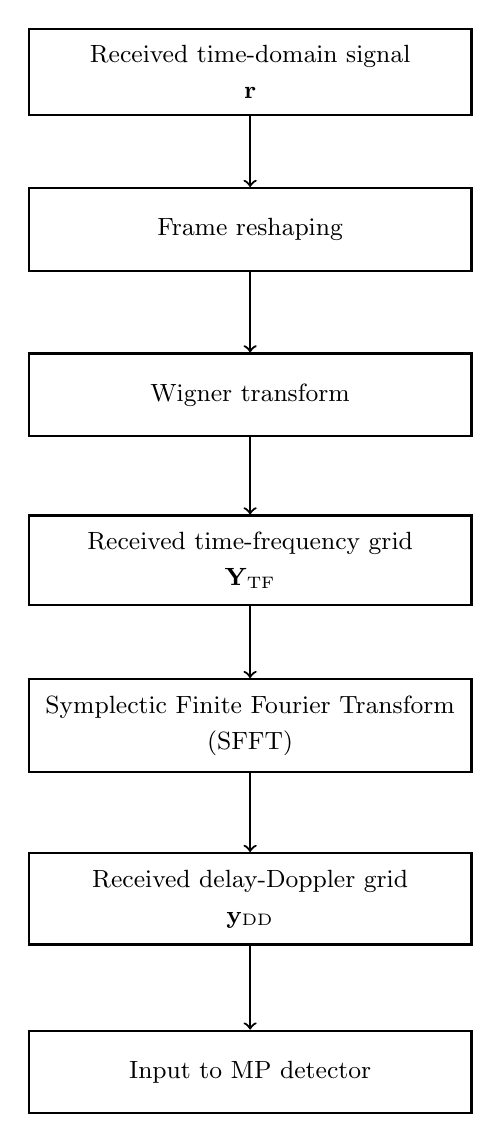
\begin{tikzpicture}[
        block/.style={
            rectangle,
            draw,
            thick,
            align=center,
            text width=5.2cm,
            minimum height=1.05cm,
            font=\small,
            inner sep=6pt
        },
        arrow/.style={
            ->,
            thick,
            shorten >=0pt,
            shorten <=0pt
        }
    ]

        \node[block] (rx) at (0,0) {Received time-domain signal\\[2pt]\(\mathbf{r}\)};
        \node[block] (reshape) at (0,-2.0) {Frame reshaping};
        \node[block] (wigner) at (0,-4.1) {Wigner transform};
        \node[block] (tf) at (0,-6.2) {Received time-frequency grid\\[2pt]\(\mathbf{Y}_{\mathrm{TF}}\)};
        \node[block] (sfft) at (0,-8.3) {Symplectic Finite Fourier Transform\\[2pt](SFFT)};
        \node[block] (dd) at (0,-10.5) {Received delay-Doppler grid\\[2pt]\(\mathbf{y}_{\mathrm{DD}}\)};
        \node[block] (detector) at (0,-12.7) {Input to MP detector};

        \draw[arrow] (rx.south) -- (reshape.north);
        \draw[arrow] (reshape.south) -- (wigner.north);
        \draw[arrow] (wigner.south) -- (tf.north);
        \draw[arrow] (tf.south) -- (sfft.north);
        \draw[arrow] (sfft.south) -- (dd.north);
        \draw[arrow] (dd.south) -- (detector.north);

    \end{tikzpicture}
    \caption{Baseline OTFS receiver processing chain}
    \label{fig:otfs_receiver_chain}
\end{figure}

Figure~\ref{fig:otfs_receiver_chain} shows that the receiver does not directly demodulate QAM symbols after the SFFT stage. This is important because the time-varying channel causes coupling among delay-Doppler symbols. Therefore, the receiver front-end only reconstructs the received delay-Doppler observation, while the actual symbol estimation is performed later by the detector.

\subsubsection{Received Signal Reshaping}

Let \(\mathbf{r}\) denote the received time-domain sample vector after the channel. This vector is reshaped into an \(M \times N\) matrix as

\begin{equation}
    \mathbf{R} = \mathrm{reshape}(\mathbf{r}, M, N).
\end{equation}

This operation restores the frame structure before applying the receiver transforms. It is the counterpart of the serialization step at the transmitter, where the time-domain transmit matrix is converted into a one-dimensional signal vector.

The reshaping operation itself does not remove channel distortion or noise. It only prepares the received samples for the Wigner transform.

\subsubsection{Wigner Transform}

The Wigner transform is used to convert the received time-domain samples into the time-frequency domain. In the discrete implementation, this operation is performed by an \(M\)-point FFT along the delay-related dimension of the reshaped received signal. The resulting time-frequency grid is denoted by \(\mathbf{Y}_{\mathrm{TF}}\).

In matrix form, the discrete Wigner stage can be represented as
\begin{equation}
    \mathbf{Y}_{\mathrm{TF}}
    =
    \left(
    \frac{1}{\sqrt{M}}\mathbf{F}_{M}\mathbf{R}
    \right)^{T},
    \label{eq:receiver_wigner_matrix}
\end{equation}
where \(\mathbf{F}_{M}\) denotes the \(M\)-point DFT matrix. The transpose follows the grid-index convention used by the transmitter-side time-frequency matrix.

The normalization factor \(\sqrt{M}\) is used to keep the signal energy consistently scaled with the transmitter implementation. After the FFT, the transpose operation arranges the matrix so that the received time-frequency samples follow the same indexing convention as the transmitted grid \(\mathbf{X}_{\mathrm{TF}}\).

Conceptually, this stage can be interpreted as the receiver counterpart of the Heisenberg transform. While the Heisenberg transform generates the time-domain waveform from the time-frequency grid, the Wigner transform extracts the time-frequency representation from the received waveform.

\subsubsection{Symplectic Finite Fourier Transform}

After obtaining the received time-frequency grid, the receiver applies the SFFT to map the signal back to the delay-Doppler domain. This is the inverse operation of the ISFFT used at the transmitter. If \(Y[n,m]\) denotes the received time-frequency sample, the corresponding delay-Doppler observation \(y[k,l]\) is obtained as

\begin{equation}
    y[k,l]
    =
    \frac{1}{\sqrt{MN}}
    \sum_{n=0}^{N-1}
    \sum_{m=0}^{M-1}
    Y[n,m]
    e^{-j2\pi\left(\frac{nk}{N}-\frac{ml}{M}\right)} .
\end{equation}

This equation is the most important receiver-side transform in the baseline OTFS model. It explains how the received signal is returned to the delay-Doppler domain, where the channel has a sparse and structured representation.

In discrete matrix processing, the SFFT combines one Fourier operation and one inverse Fourier operation along the two OTFS grid dimensions. The normalization term is selected consistently with the transmitter-side ISFFT normalization, ensuring that the overall modulation and demodulation chain has compatible energy scaling.

\subsubsection{Received Delay-Doppler Observation}

The output of the OTFS demodulator is the received delay-Doppler grid \(\mathbf{y}_{\mathrm{DD}}\). In an ideal channel without noise or Doppler-delay spreading, this grid would match the transmitted delay-Doppler symbol grid. In the simulated doubly dispersive channel, however, each received grid point may contain contributions from several transmitted symbols due to delay shifts, Doppler shifts, and complex fading coefficients.

Therefore, the received delay-Doppler grid should be understood as an observation, not as a final decision. The receiver front-end produces

\begin{equation}
    \mathbf{y}_{\mathrm{DD}} = \mathrm{SFFT}\left\{\mathbf{Y}_{\mathrm{TF}}\right\},
\end{equation}

and this observation is then passed to the message passing detector. The detector uses the channel information, delay taps, Doppler taps, and path coefficients to estimate the transmitted QAM symbols.

This separation between demodulation and detection is important in OTFS. The demodulator only changes the signal representation, while the detector resolves the interference introduced by the time-varying multipath channel.

\subsubsection{Discrete Receiver Processing Summary}

The complete receiver front-end can be summarized by the ordered sequence
\begin{equation}
    \mathbf{r}
    \xrightarrow{\text{frame reshaping}}
    \mathbf{R}
    \xrightarrow{\text{Wigner transform}}
    \mathbf{Y}_{\mathrm{TF}}
    \xrightarrow{\text{SFFT}}
    \mathbf{y}_{\mathrm{DD}} .
    \label{eq:receiver_discrete_summary}
\end{equation}
The first operation restores the received OTFS frame. The Wigner transform then extracts the time-frequency grid, and the SFFT returns the observation to the delay-Doppler domain.

This processing order is consistent with the transmitter chain. The transmitter maps delay-Doppler symbols to the time-frequency domain using the ISFFT and then generates the time-domain signal using the Heisenberg transform. The receiver reverses this order by first applying the Wigner transform and then the SFFT.

\subsubsection{Summary of the Baseline OTFS Receiver}

The baseline OTFS receiver converts the received time-domain waveform back into a delay-Doppler observation through two main operations. The Wigner transform extracts the time-frequency grid from the received samples, and the SFFT maps this grid into the delay-Doppler domain. The receiver output is not yet the estimated transmitted data, because the delay-Doppler symbols are still affected by channel-induced interference.

The overall receiver front-end can be summarized as

\begin{equation}
    \mathbf{r}
    \rightarrow
    \mathbf{R}
    \rightarrow
    \mathbf{Y}_{\mathrm{TF}}
    \rightarrow
    \mathbf{y}_{\mathrm{DD}} .
\end{equation}

The delay-Doppler observation \(\mathbf{y}_{\mathrm{DD}}\) is then used as the input to the message passing detector. This completes the receiver-side signal transformation and prepares the system for symbol estimation, which is discussed in the following sections.


\subsection{Equivalent Input-Output Model for Detection}

After OTFS demodulation, the receiver obtains the delay-Doppler observation grid \(\mathbf{y}_{\mathrm{DD}}\). This grid is not yet the final estimate of the transmitted symbols because the doubly dispersive channel introduces interference among delay-Doppler positions. At the grid level, the received delay-Doppler sample can be interpreted as a two-dimensional circular convolution between the transmitted symbols and the sparse delay-Doppler channel. A compact form of this relation is

\begin{equation}
    y[k,l]
    =
    \sum_{i=1}^{P}
    h_i
    x\!\left([\!k-\nu_i\!]_N,[\!l-l_i\!]_M\right)
    +
    w[k,l],
    \label{eq:dd_2d_convolution}
\end{equation}

where \(P\) is the number of channel paths, \(h_i\) is the complex gain of the \(i\)-th path, \(\nu_i\) and \(l_i\) denote the Doppler and delay shifts, and \([\cdot]_N\) and \([\cdot]_M\) denote circular indexing over the Doppler and delay dimensions, respectively. This expression shows that the received sample at one delay-Doppler position may contain contributions from several shifted transmitted symbols.

For detection, the two-dimensional delay-Doppler grid is rewritten into an equivalent vector input-output model. Let \(\mathbf{x}\) denote the transmitted delay-Doppler symbol vector and \(\mathbf{y}\) denote the received delay-Doppler observation vector. Both vectors have length \(MN\), where \(M\) is the number of delay bins and \(N\) is the number of Doppler bins. The equivalent input-output relation can be written as

\begin{equation}
    \mathbf{y}
    =
    \mathbf{H}_{\mathrm{DD}}\mathbf{x}
    +
    \mathbf{w},
    \label{eq:dd_input_output_model}
\end{equation}

where \(\mathbf{H}_{\mathrm{DD}}\) is the effective delay-Doppler channel matrix and \(\mathbf{w}\) is the additive noise vector after demodulation.

Equation~\eqref{eq:dd_input_output_model} is the key model used for detection. It shows that each received delay-Doppler sample is a linear combination of transmitted symbols affected by the channel. If the channel contained only a single zero-delay and zero-Doppler path, \(\mathbf{H}_{\mathrm{DD}}\) would reduce to a scaled identity-like matrix. In a time-varying multipath channel, however, delay and Doppler shifts move the transmitted symbols across the delay-Doppler grid, so the channel matrix contains structured off-diagonal components.

\subsubsection{Vector Representation of the Delay-Doppler Grid}

The transmitted delay-Doppler grid is first arranged as a two-dimensional matrix of size \(N \times M\). Equivalently, the QAM symbol vector is mapped into a fixed \(N \times M\) delay-Doppler ordering before detection.

For detection, the same grid can be represented as a vector. If \(x[k,l]\) denotes the symbol at Doppler index \(k\) and delay index \(l\), the corresponding vector element can be written as

\begin{equation}
    x_{q} = x[k,l],
    \qquad
    q = k + lN .
\end{equation}

The received delay-Doppler grid is vectorized in the same way. This vector representation is useful because the detector operates on indexed symbol positions rather than on a purely visual two-dimensional grid.

\subsubsection{Sparse Structure of the Delay-Doppler Channel}

The delay-Doppler channel matrix \(\mathbf{H}_{\mathrm{DD}}\) is sparse because the simulated channel contains only a limited number of propagation paths. Each path is characterized by a delay tap, a Doppler tap, and a complex fading coefficient. As a result, each transmitted symbol only contributes significantly to a small number of received positions.

This sparse structure is important for the message passing detector. Instead of treating every transmitted symbol as interfering with every received symbol, the detector only needs to consider the dominant connections created by the channel taps. This reduces the detection complexity compared with a full exhaustive search over all possible transmitted symbol vectors.

In the simulation, this structure is not explicitly stored as a full dense matrix. Instead, the detector uses the delay taps, Doppler taps, and channel coefficients directly. This avoids unnecessary memory usage and matches the sparse physical interpretation of the delay-Doppler channel.

\subsubsection{Role of the Equivalent Model in the Receiver}

The equivalent input-output model separates the receiver into two conceptual parts. The first part is the OTFS demodulator, which converts the received waveform into the delay-Doppler observation \(\mathbf{y}\). The second part is the detector, which estimates the transmitted symbol vector \(\mathbf{x}\) based on \(\mathbf{y}\) and the channel information.

This separation is useful because the demodulation stage only performs deterministic signal transformations, while the detection stage deals with channel-induced interference and noise. Therefore, the model in Equation~\eqref{eq:dd_input_output_model} provides the direct mathematical foundation for the message passing detector discussed in the next section.

\subsubsection{Summary of the Detection Model}

The baseline OTFS receiver can be summarized by the following delay-Doppler input-output relation:

\begin{equation}
    \mathbf{y}
    =
    \mathbf{H}_{\mathrm{DD}}\mathbf{x}
    +
    \mathbf{w}.
\end{equation}

This model shows that the received delay-Doppler vector is affected by the sparse time-varying channel and additive noise. It also explains why a dedicated detector is required after OTFS demodulation. The next section presents the message passing detector used to estimate the transmitted QAM symbols from this equivalent delay-Doppler model.


\subsection{Message Passing Detector Design}

After OTFS demodulation, the receiver obtains the delay-Doppler observation vector \(\mathbf{y}\). Because the channel is time-varying and multipath, each received delay-Doppler sample may contain contributions from several transmitted symbols. A direct exhaustive search over all possible transmitted symbol vectors would be computationally impractical. Therefore, the baseline OTFS receiver uses a message passing detector to estimate the transmitted QAM symbols from the sparse delay-Doppler input-output model.

The detector used in this thesis follows the message passing structure commonly adopted for OTFS detection over sparse delay-Doppler channels. The same detector core is later reused for OTFS-IM. In the baseline OTFS case, the detector output is used to form hard QAM symbol decisions. In the OTFS-IM case, the probability output of the same detector is further processed to detect both active positions and QAM symbols, as discussed in Chapter 4.

\subsubsection{Motivation for Message Passing Detection}

From Section 3.5, the equivalent delay-Doppler input-output relation can be written as
\begin{equation}
    \mathbf{y}
    =
    \mathbf{H}_{\mathrm{DD}}\mathbf{x}
    +
    \mathbf{w}.
\end{equation}
The matrix \(\mathbf{H}_{\mathrm{DD}}\) is sparse because the channel contains only a limited number of delay-Doppler paths. This means that each received symbol is mainly affected by a small subset of transmitted symbols, rather than by all \(MN\) transmitted symbols.

This sparse structure makes message passing suitable for OTFS detection. Instead of solving the full linear system using a dense matrix inversion, the detector iteratively exchanges probability information between received observation nodes and transmitted symbol nodes. The algorithm estimates the probability that each transmitted symbol belongs to each constellation point, and then makes a hard decision after the probabilities converge or the maximum number of iterations is reached.

\begin{figure}[H]
    \centering
    \begin{tikzpicture}[
        startstop/.style={
            rectangle,
            rounded corners,
            draw,
            thick,
            align=center,
            text width=5.4cm,
            minimum height=0.72cm,
            font=\footnotesize,
            inner sep=4pt
        },
        io/.style={
            trapezium,
            trapezium left angle=70,
            trapezium right angle=110,
            draw,
            thick,
            align=center,
            text width=5.2cm,
            minimum height=0.72cm,
            font=\footnotesize,
            inner sep=4pt
        },
        process/.style={
            rectangle,
            draw,
            thick,
            align=center,
            text width=5.9cm,
            minimum height=0.72cm,
            font=\footnotesize,
            inner sep=4pt
        },
        decision/.style={
            diamond,
            draw,
            thick,
            align=center,
            text width=2.7cm,
            aspect=1.85,
            font=\footnotesize,
            inner sep=1pt
        },
        arrow/.style={
            ->,
            thick
        }
    ]

        \node[io] (input) at (0,0) {Input \(\mathbf{y}\), channel taps, channel gains, \(\sigma^2\)};
        \node[process] (init) at (0,-1.50) {Initialize candidate alphabet and uniform probabilities};
        \node[process] (meanvar) at (0,-3.00) {Observation-node update: compute interference mean and variance};
        \node[process] (prob) at (0,-4.50) {Variable-node update: compute likelihoods and symbol probabilities};
        \node[process] (damp) at (0,-6.00) {Apply damping to stabilize probability updates};
        \node[decision] (conv) at (0,-8.05) {Converged or max iterations?};
        \node[startstop] (hard) at (0,-10.35) {Hard decision and final probability output};

        \draw[arrow] (input.south) -- (init.north);
        \draw[arrow] (init.south) -- (meanvar.north);
        \draw[arrow] (meanvar.south) -- (prob.north);
        \draw[arrow] (prob.south) -- (damp.north);
        \draw[arrow] (damp.south) -- (conv.north);
        \draw[arrow] (conv.south) -- node[right, font=\footnotesize, pos=0.45] {Yes} (hard.north);
        \draw[arrow] (conv.east) -- ++(2.25,0) |- node[pos=0.25, right, font=\footnotesize] {No} (meanvar.east);

    \end{tikzpicture}
    \caption{Operational flow of the message passing detector}
    \label{fig:mp_detector_flow}
\end{figure}

Figure~\ref{fig:mp_detector_flow} summarizes the operational flow of the detector. The algorithm starts with uniform symbol probabilities, repeatedly refines the interference statistics and symbol probabilities, and stops when the probability decisions become sufficiently reliable or when the iteration limit is reached.

\subsubsection{Sparse Factor-Graph Interpretation}

The message passing detector can be interpreted using a factor graph. In this graph, variable nodes represent transmitted symbols, while observation nodes represent received delay-Doppler samples. An edge exists between a variable node and an observation node if the corresponding transmitted symbol contributes to that received sample through one of the channel taps.

\begin{figure}[H]
    \centering
    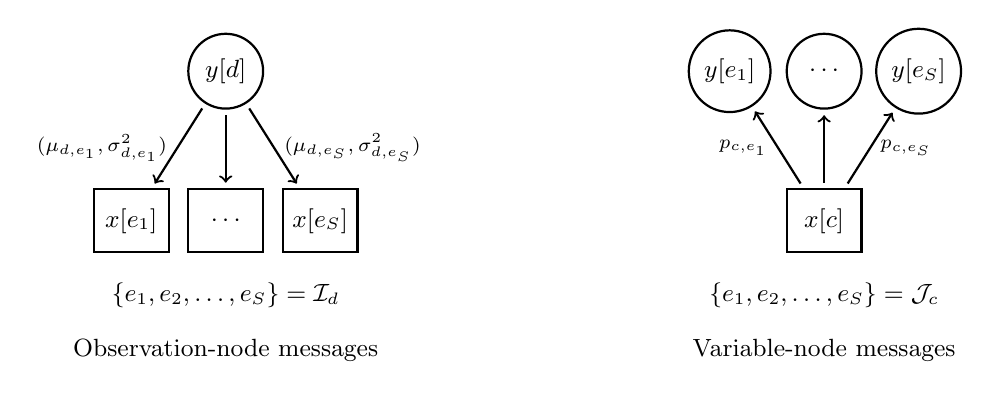
\begin{tikzpicture}[
        obsnode/.style={
            circle,
            draw,
            thick,
            align=center,
            minimum size=0.95cm,
            font=\small
        },
        varnode/.style={
            rectangle,
            draw,
            thick,
            align=center,
            minimum width=0.95cm,
            minimum height=0.8cm,
            font=\small
        },
        arrow/.style={
            ->,
            thick,
            shorten >=2pt,
            shorten <=2pt
        }
    ]

        % Observation-node messages
        \node[obsnode] (yd) at (-3.8,0.3) {\(y[d]\)};
        \node[varnode] (xe1) at (-5.0,-1.6) {\(x[e_1]\)};
        \node[varnode] (xe2) at (-3.8,-1.6) {\(\cdots\)};
        \node[varnode] (xes) at (-2.6,-1.6) {\(x[e_S]\)};

        \draw[arrow] (yd) -- node[left, font=\scriptsize, pos=0.52]
            {\((\mu_{d,e_1},\sigma^2_{d,e_1})\)} (xe1);
        \draw[arrow] (yd) -- (xe2);
        \draw[arrow] (yd) -- node[right, font=\scriptsize, pos=0.52]
            {\((\mu_{d,e_S},\sigma^2_{d,e_S})\)} (xes);

        \node[align=center, font=\small] at (-3.8,-2.55)
            {\(\{e_1,e_2,\ldots,e_S\}=\mathcal{I}_d\)};
        \node[align=center, font=\small] at (-3.8,-3.25)
            {Observation-node messages};

        % Variable-node messages
        \node[varnode] (xc) at (3.8,-1.6) {\(x[c]\)};
        \node[obsnode] (ye1) at (2.6,0.3) {\(y[e_1]\)};
        \node[obsnode] (ye2) at (3.8,0.3) {\(\cdots\)};
        \node[obsnode] (yes) at (5.0,0.3) {\(y[e_S]\)};

        \draw[arrow] (xc) -- node[left, font=\scriptsize, pos=0.50]
            {\(p_{c,e_1}\)} (ye1);
        \draw[arrow] (xc) -- (ye2);
        \draw[arrow] (xc) -- node[right, font=\scriptsize, pos=0.50]
            {\(p_{c,e_S}\)} (yes);

        \node[align=center, font=\small] at (3.8,-2.55)
            {\(\{e_1,e_2,\ldots,e_S\}=\mathcal{J}_c\)};
        \node[align=center, font=\small] at (3.8,-3.25)
            {Variable-node messages};

    \end{tikzpicture}
    \caption{Observation-node and variable-node messages in the MP detector}
    \label{fig:mp_factor_graph}
\end{figure}

Figure~\ref{fig:mp_factor_graph} illustrates the two types of messages exchanged in the MP detector. An observation node \(y[d]\) sends interference statistics, represented by the mean and variance pair \((\mu_{d,e},\sigma^2_{d,e})\), to its neighboring variable nodes. Conversely, a variable node \(x[c]\) sends probability messages \(p_{c,e}\) to the observation nodes connected to it. The neighbor sets \(\mathcal{I}_d\) and \(\mathcal{J}_c\) are determined by the delay taps, Doppler taps, and channel coefficients. Since the number of paths is small, each node is connected only to a limited number of neighboring nodes. This locality is the main reason why message passing can reduce the detection complexity.

\begin{algorithm}[H]
    \caption{Message passing detector for OTFS symbol detection}
    \label{alg:mp_detector}
    \begin{algorithmic}[1]
        \REQUIRE Received delay-Doppler vector \(\mathbf{y}\), delay taps, Doppler taps, channel coefficients, noise variance \(\sigma^2\), candidate alphabet \(\mathcal{A}_{0}\)
        \ENSURE Hard symbol estimate \(\widehat{\mathbf{x}}\) and final probability map
        \STATE Vectorize the received grid as \(\mathbf{y}=\mathrm{vec}(\mathbf{y}_{\mathrm{DD}})\)
        \STATE Initialize all symbol probabilities uniformly over \(\mathcal{A}_{0}\)
        \FOR{\(i=1\) to \(N_{\mathrm{ite}}\)}
            \STATE For each observation-symbol connection, compute the effective channel coefficient from the delay and Doppler taps
            \STATE Compute the interference mean by excluding the candidate symbol being updated
            \STATE Compute the interference variance and add the noise variance \(\sigma^2\)
            \STATE Evaluate the likelihood of every candidate symbol in \(\mathcal{A}_{0}\)
            \STATE Normalize the likelihoods to obtain updated symbol probabilities
            \STATE Apply damping between the new probabilities and the previous probabilities
            \STATE Compute the convergence rate from the maximum probability at each symbol position
            \IF{all symbol positions are reliable or the convergence rate degrades}
                \STATE Stop the iteration
            \ENDIF
        \ENDFOR
        \STATE Select the symbol with the largest final probability at each position
        \RETURN \(\widehat{\mathbf{x}}\) and the final probability map
    \end{algorithmic}
\end{algorithm}

Algorithm~\ref{alg:mp_detector} presents the computational order of the detector. The most important idea is that the detector does not decide symbols immediately after OTFS demodulation. Instead, it repeatedly estimates the interference caused by neighboring delay-Doppler symbols and uses this estimate to refine the probability of each candidate symbol.

\subsubsection{Algorithmic Complexity Interpretation}

The advantage of message passing becomes clearer when it is compared with an exhaustive detector. If all \(MN\) transmitted OTFS symbols were detected jointly, the search space would grow as \(|\mathcal{A}|^{MN}\), where \(|\mathcal{A}|\) is the constellation size. This is impossible even for moderate frame sizes. For the baseline setup in this thesis, \(MN=120\), so a full joint search over 4-QAM candidates would require \(4^{120}\) possible symbol vectors. This number is far beyond practical simulation or implementation.

The MP detector avoids this full search by using the sparse delay-Doppler channel structure. Since each received observation is connected only to a limited number of transmitted symbols, the detector updates probabilities locally rather than globally. If the number of channel paths is \(P\), the number of detector iterations is \(N_{\mathrm{ite}}\), and the candidate alphabet size is \(|\mathcal{A}_{0}|\), a useful high-level complexity description is
\begin{equation}
    \mathcal{O}
    \left(
    N_{\mathrm{ite}}
    MN
    P
    |\mathcal{A}_{0}|
    \right).
    \label{eq:mp_complexity_order}
\end{equation}
This expression is not intended to count every arithmetic operation exactly. Its purpose is to show the scaling behavior: the computational effort grows approximately linearly with the number of delay-Doppler resource elements, the number of channel paths, the number of iterations, and the number of candidate symbols.

This complexity interpretation also explains why the same detector can be reused for OTFS-IM. In OTFS-IM, the alphabet is extended by adding the inactive symbol \(0\). Therefore, the detector does not need a different factor-graph structure. It only evaluates one additional candidate state per resource element. The more difficult OTFS-IM operation is not the MP update itself, but the block-wise interpretation of the resulting probability map, which is developed in Chapter 4.

From a reporting perspective, this distinction is important. The MP detector provides a soft reliability profile over the delay-Doppler grid. The later OTFS-IM receiver then uses this reliability profile to decide which positions are active. Therefore, the detector is not only a symbol estimator; it is also the probability engine that enables index detection.

\subsubsection{Role of Damping and Stopping in the Iterative Process}

The damping factor is included because probability messages in a loopy factor graph can oscillate between iterations. In an ideal tree-structured factor graph, messages can converge in a finite number of passes. The OTFS detection graph, however, contains cycles because several transmitted symbols can affect several received observations through different delay-Doppler shifts. In this case, updating probabilities too aggressively may cause the detector to overreact to an unreliable intermediate estimate.

Damping reduces this problem by mixing the newly computed probability with the previous probability. A large damping factor gives more weight to the new likelihood information and can lead to faster convergence when the observation is reliable. A smaller damping factor makes the detector more conservative and can improve stability when the received observation is noisy or when the interference estimate is still inaccurate. The value \(\Delta=0.6\) used in the simulation therefore represents a compromise between convergence speed and numerical stability.

The convergence criterion is also important. The detector does not need to run the full number of iterations if most symbol probabilities have already become reliable. In this thesis, reliability is measured by checking whether the largest candidate probability at a symbol position exceeds a high threshold. If the maximum probability is close to one, the detector is confident about that symbol decision. If many positions remain uncertain, additional iterations may still improve the probability map.

However, more iterations do not always guarantee better BER. In a loopy message-passing detector, later iterations can sometimes reinforce an incorrect decision if the probability map becomes overconfident too early. For this reason, the stopping rule also monitors whether the convergence behavior is improving. The detector is therefore designed to stop when the probability map has become sufficiently reliable or when further iterations are unlikely to provide useful improvement.

\begin{table}[H]
\centering
\caption{Interpretation of key MP detector parameters.}
\label{tab:mp_detector_parameter_roles}
\begin{tabularx}{0.95\linewidth}{|p{3.0cm}|X|}
\hline
\textbf{Parameter} & \textbf{Role in the detector} \\
\hline
\(P\) & Number of channel paths; determines how many neighboring symbols contribute significantly to each observation. \\
\hline
\(|\mathcal{A}_{0}|\) & Number of candidate symbol states; includes QAM symbols and, for OTFS-IM reuse, the inactive zero state. \\
\hline
\(N_{\mathrm{ite}}\) & Maximum number of message-passing iterations; limits complexity and prevents endless updates. \\
\hline
\(\Delta\) & Damping factor; balances new probability information and previous messages to improve stability. \\
\hline
\(\sigma^2\) & Noise variance; affects the likelihood width and therefore the confidence of probability updates. \\
\hline
\end{tabularx}
\end{table}

Table~\ref{tab:mp_detector_parameter_roles} also shows why detector parameters must be reported together with BER results. If the number of iterations, damping factor, or noise normalization were changed, the detector output probabilities could change even under the same channel realization. Keeping these parameters fixed is therefore necessary for a fair comparison between baseline OTFS and OTFS-IM.

\subsubsection{Symbol Alphabet and Probability Initialization}

Let \(\mathcal{A}\) denote the QAM constellation alphabet. For baseline OTFS with 4-QAM, \(\mathcal{A}\) contains four constellation points. The detector estimates, for each transmitted symbol position, the probability that the symbol belongs to each element of the alphabet.

To make the detector reusable for both baseline OTFS and OTFS-IM, an extended candidate alphabet is defined as
\begin{equation}
    \mathcal{A}_{0}
    =
    \mathcal{A}
    \cup
    \{0\}.
\end{equation}
The zero symbol is included because the same detector is later used for OTFS-IM, where inactive positions correspond to zero-valued transmitted symbols. For the baseline OTFS discussion, the important point is that the detector produces symbol probabilities over the candidate alphabet. The probability output is then used either for direct hard QAM decisions in baseline OTFS or for block-wise index detection in OTFS-IM.

At the beginning of the algorithm, all symbol candidates are assigned equal probability:
\begin{equation}
    p_{c,d}^{(0)}(a_j)
    =
    \frac{1}{|\mathcal{A}_{0}|},
    \qquad
    a_j\in\mathcal{A}_{0}.
    \label{eq:mp_uniform_initialization}
\end{equation}
This initialization avoids biasing the first iteration toward any constellation point or inactive state.

\subsubsection{Observation-Node Mean and Variance Update}

Consider one received observation \(y[d]\) and one transmitted symbol \(x[c]\) connected to it. The received sample can be written as
\begin{equation}
    y[d]
    =
    H[d,c]x[c]
    +
    \sum_{e\in\mathcal{I}(d),\,e\neq c}
    H[d,e]x[e]
    +
    w[d],
    \label{eq:mp_observation_model}
\end{equation}
where \(\mathcal{I}(d)\) is the set of transmitted symbols connected to observation node \(d\). The summation term represents the interference caused by other connected symbols.

In message passing detection, this interference is approximated as a Gaussian random variable. Therefore, for each connected edge, the observation node computes the mean and variance of the interference using the current symbol probabilities. If \(p_{e,d}^{(i-1)}(a_j)\) is the probability from the previous iteration that \(x[e]=a_j\), the interference mean can be expressed as
\begin{equation}
    \mu_{d,c}^{(i)}
    =
    \sum_{e\in\mathcal{I}(d),\,e\neq c}
    \sum_{a_j\in\mathcal{A}_{0}}
    p_{e,d}^{(i-1)}(a_j)
    a_j
    H[d,e].
\end{equation}
The corresponding variance is
\begin{equation}
    \begin{aligned}
    \left(\sigma_{d,c}^{(i)}\right)^2
    &=
    \sum_{e\in\mathcal{I}(d),\,e\neq c}
    \Bigg(
    \sum_{a_j\in\mathcal{A}_{0}}
    p_{e,d}^{(i-1)}(a_j)
    |a_j|^2
    |H[d,e]|^2
    \\
    &\qquad
    -
    \left|
    \sum_{a_j\in\mathcal{A}_{0}}
    p_{e,d}^{(i-1)}(a_j)
    a_j
    H[d,e]
    \right|^2
    \Bigg)
    +
    \sigma^2.
    \end{aligned}
\end{equation}
These two quantities summarize the contribution of all interfering symbols except the candidate symbol currently being updated.

\subsubsection{Variable-Node Probability Update with Damping}

After the observation-node update, the detector updates the probability of each candidate symbol. For a candidate value \(a_j\), the likelihood is computed by comparing the received observation with the predicted contribution of \(a_j\), while treating the remaining interference as Gaussian. A compact likelihood expression is
\begin{equation}
    \xi^{(i)}(d,c,a_j)
    =
    \exp
    \left(
    -
    \frac{
    \left|
    y[d]
    -
    \mu_{d,c}^{(i)}
    -
    H[d,c]a_j
    \right|^2
    }{
    \left(\sigma_{d,c}^{(i)}\right)^2
    }
    \right).
\end{equation}
The probability of each candidate symbol is then updated using the product of the likelihoods from the connected observation nodes. This follows the standard message passing principle that a variable node combines information from its neighboring observation nodes.

For numerical stability, the probability update can be evaluated in the logarithmic domain. After the new probability is computed, damping is applied:
\begin{equation}
    p_{c,d}^{(i)}(a_j)
    =
    \Delta \widetilde{p}_{c,d}^{(i)}(a_j)
    +
    (1-\Delta)p_{c,d}^{(i-1)}(a_j),
    \label{eq:mp_damping}
\end{equation}
where \(\widetilde{p}_{c,d}^{(i)}(a_j)\) is the newly computed probability and \(\Delta\) is the damping factor. In the simulation, the damping factor is set to
\begin{equation}
    \Delta = 0.6.
\end{equation}
Damping prevents the probabilities from changing too aggressively between iterations. This helps stabilize the iterative detector, especially when the factor graph contains cycles.

\subsubsection{Hard Decision and Convergence Criterion}

At each iteration, the detector computes the final symbol probability for every transmitted position. The hard decision is obtained by selecting the candidate symbol with the largest probability:
\begin{equation}
    j^{\star}
    =
    \arg\max_{j}
    p_c(a_j).
\end{equation}
The detected symbol is then
\begin{equation}
    \widehat{x}[c] = a_{j^{\star}}.
    \label{eq:mp_hard_decision}
\end{equation}

The implementation also evaluates a convergence indicator. A symbol position is considered reliable if the maximum probability exceeds \(0.99\). The convergence rate is therefore computed as the fraction of symbol positions satisfying this condition:
\begin{equation}
    \eta^{(i)}
    =
    \frac{1}{MN}
    \sum_{c=1}^{MN}
    \mathbf{1}
    \left(
    \max_{a_j\in\mathcal{A}_{0}} p_c^{(i)}(a_j) > 0.99
    \right).
\end{equation}
If all positions become reliable, the detector stops early. Otherwise, the algorithm continues until the maximum number of iterations is reached. In the simulation, the maximum number of message passing iterations is
\begin{equation}
    N_{\mathrm{ite}} = 10.
\end{equation}

\subsubsection{Detector Input and Output Summary}

The detector takes the received delay-Doppler observation, the OTFS frame size, the QAM order, the delay and Doppler taps, the channel coefficients, and the noise variance as its main inputs. The received grid is first vectorized so that each delay-Doppler position can be treated as one variable node in the factor graph:
\begin{equation}
    \mathbf{y}_{v}
    =
    \mathrm{vec}\!\left(\mathbf{y}_{\mathrm{DD}}\right).
    \label{eq:mp_received_vectorization}
\end{equation}
The detector then initializes the probability map, iteratively updates the interference mean and variance, updates the symbol probabilities with damping, and finally returns both a hard symbol estimate and a final probability map. The hard estimate is denoted by \(\widehat{\mathbf{x}}\), while the final probability map is denoted by \(\mathbf{P}_{\mathrm{fin}}\).

For the baseline OTFS system, \(\widehat{\mathbf{x}}\) is used to recover the QAM symbols and compute the BER. For the OTFS-IM system in Chapter 4, \(\mathbf{P}_{\mathrm{fin}}\) becomes especially important because it provides the probability that each position is active or inactive. The OTFS-IM receiver then uses these probabilities to perform block-wise pattern detection. Therefore, the detector described in this section is a common receiver component shared by both the baseline OTFS and OTFS-IM systems.

\subsubsection{Summary of the Detector Design}

The message passing detector exploits the sparse structure of the delay-Doppler channel. Instead of solving the full detection problem by exhaustive search, it iteratively exchanges probability information between received observation nodes and transmitted symbol nodes. The observation-node update computes the mean and variance of the interference, while the variable-node update refines the probability of each candidate symbol.

In the baseline OTFS receiver, the detector produces hard QAM symbol decisions used for BER evaluation. In the later OTFS-IM receiver, the same probability output is reused to detect active-position patterns and QAM symbols jointly at the block level. This makes the MP detector a central component of the simulation framework and provides the receiver foundation for the OTFS-IM design developed in Chapter 4.


\subsection{OTFS Simulation Flow}

The previous sections have described the baseline OTFS system from the transmitter, channel, receiver, input-output model, and detector perspectives. This section connects these individual processing blocks into the end-to-end simulation flow used for BER evaluation. The purpose is not to introduce a new theoretical model, but to clarify how the baseline OTFS chain is executed in MATLAB before it is used as a reference system in the performance evaluation chapter.

In the simulation framework, the baseline OTFS system is evaluated through an end-to-end Monte Carlo loop. For each value of \(E_b/N_0\), the simulator generates random information bits, maps them into QAM symbols, places the symbols on the delay-Doppler grid, applies OTFS modulation, passes the transmitted signal through the delay-Doppler multipath channel, performs OTFS demodulation, detects the transmitted symbols using the MP detector, and finally computes the BER by comparing the detected bits with the transmitted bits.

\begin{figure}[H]
    \centering
    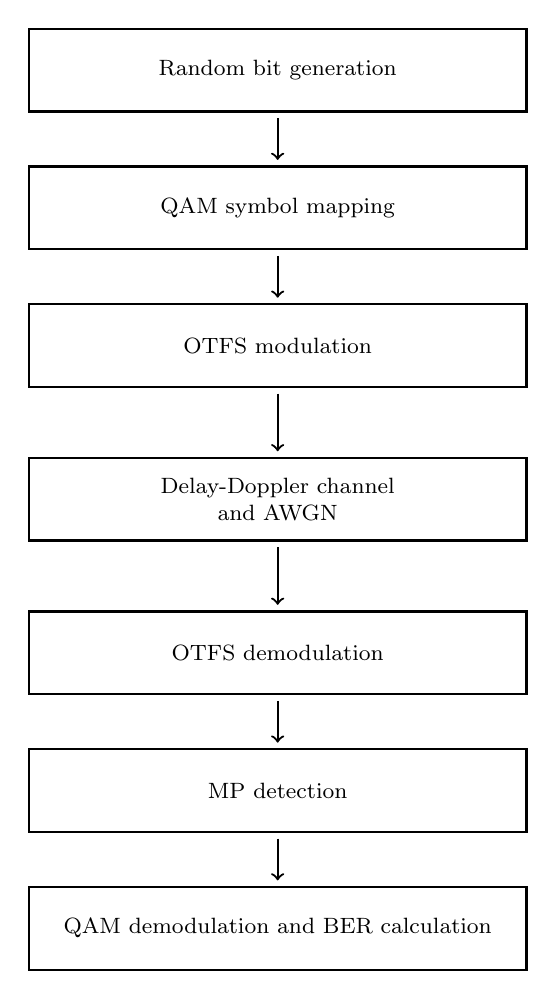
\begin{tikzpicture}[
        block/.style={
            rectangle,
            draw,
            thick,
            align=center,
            text width=5.9cm,
            minimum height=1.05cm,
            font=\footnotesize,
            inner sep=6pt
        },
        arrow/.style={
            ->,
            thick,
            shorten >=2pt,
            shorten <=2pt
        }
    ]

        \node[block] (bits) at (0,0) {Random bit generation};
        \node[block] (qam) at (0,-1.75) {QAM symbol mapping};
        \node[block] (mod) at (0,-3.50) {OTFS modulation};
        \node[block] (chan) at (0,-5.45) {Delay-Doppler channel\\and AWGN};
        \node[block] (demod) at (0,-7.40) {OTFS demodulation};
        \node[block] (mp) at (0,-9.15) {MP detection};
        \node[block] (ber) at (0,-10.90) {QAM demodulation and BER calculation};

        \draw[arrow] (bits.south) -- (qam.north);
        \draw[arrow] (qam.south) -- (mod.north);
        \draw[arrow] (mod.south) -- (chan.north);
        \draw[arrow] (chan.south) -- (demod.north);
        \draw[arrow] (demod.south) -- (mp.north);
        \draw[arrow] (mp.south) -- (ber.north);

    \end{tikzpicture}
    \caption{Baseline OTFS simulation flow used for BER evaluation}
    \label{fig:baseline_otfs_simulation_flow}
\end{figure}

Figure~\ref{fig:baseline_otfs_simulation_flow} summarizes the simulation flow. The first stage creates an equiprobable binary information sequence
\begin{equation}
    \mathbf{b}
    \in
    \{0,1\}^{N_{\mathrm{bits}}},
    \qquad
    \Pr(b_i=0)=\Pr(b_i=1)=\frac{1}{2}.
    \label{eq:baseline_random_bits}
\end{equation}
The generated bits are then grouped according to the QAM order and mapped to complex QAM symbols. For the baseline OTFS case, all delay-Doppler positions carry QAM symbols, because no index modulation is applied at this stage.

The mapped QAM symbols are reshaped into the \(N\times M\) delay-Doppler grid and processed by the OTFS transmitter described in Section 3.2. The output is a time-domain transmit vector. A channel realization is then generated by specifying the number of paths, delay taps, Doppler taps, and complex channel coefficients. The transmitted signal is passed through this time-varying multipath channel and corrupted by AWGN.

At the receiver, OTFS demodulation transforms the received time-domain signal back to the delay-Doppler observation grid. The MP detector then estimates the transmitted symbols from this observation using the sparse delay-Doppler channel structure. The estimated QAM symbols are demodulated back into bits, and the BER is computed as
\begin{equation}
    \mathrm{BER}
    =
    \frac{N_{\mathrm{err}}}{N_{\mathrm{bits}}},
\end{equation}
where \(N_{\mathrm{err}}\) is the number of incorrectly detected bits and \(N_{\mathrm{bits}}\) is the total number of transmitted bits over the simulated frames.

The baseline OTFS simulation also supports adaptive stopping in the Monte Carlo loop. If adaptive simulation is enabled, the number of frames at a given \(E_b/N_0\) point can stop early after a minimum number of frames and a target number of bit errors have been reached. This keeps the simulation practical while still collecting enough errors for BER estimation. If adaptive simulation is not enabled, the simulator uses the fixed number of frames specified in the configuration.

The baseline OTFS simulation outputs include the accumulated bit errors, the number of frames used at each SNR point, and the resulting BER vector. These outputs are later combined with the OFDM, OTFS-IM, and pattern-selection results in the main experiment runner. Therefore, the baseline OTFS flow provides the reference BER curve against which the proposed OTFS-IM schemes are evaluated in Chapter 5.


\subsection{Design Discussion and Chapter Summary}

This chapter has developed the baseline OTFS system used as the foundation for the later OTFS-IM design. The main design idea is to represent information symbols in the delay-Doppler domain, transform them to the time-frequency domain for transmission, and recover them through an OTFS receiver followed by message passing detection. This structure is suitable for time-varying multipath channels because the dominant propagation effects can be represented through a limited number of delay and Doppler taps.

The baseline system is intentionally kept as a conventional OTFS chain without index modulation. This is important for two reasons. First, it provides a clean reference that shows the performance of OTFS modulation and MP detection under the same delay-Doppler channel model used later in the thesis. Second, it allows the contribution of OTFS-IM to be evaluated separately. If index modulation were introduced too early, it would be difficult to distinguish between the benefit of the OTFS waveform itself and the effect of activating only selected positions within each IM block.

From a transmitter perspective, the baseline system maps QAM symbols directly onto the full delay-Doppler grid. The ISFFT and Heisenberg transform then produce the transmit signal. From a channel perspective, the simulation uses a discrete delay-Doppler multipath model with delay taps, Doppler taps, complex Rayleigh fading coefficients, and AWGN. From a receiver perspective, the received signal is transformed back to the delay-Doppler domain and detected using the MP detector. These blocks form a complete baseline chain that can be simulated repeatedly over different \(E_b/N_0\) values to obtain BER performance.

The use of the MP detector is a key part of the baseline receiver. A direct exhaustive search over all possible transmitted symbol vectors would be computationally expensive, especially as the frame size increases. The sparse delay-Doppler channel structure makes message passing more suitable because each received observation is connected to only a limited number of transmitted symbols. The detector therefore provides both hard symbol estimates and probability outputs. In the baseline OTFS system, the hard estimates are sufficient for BER calculation. In the OTFS-IM system developed in the next chapter, the probability outputs become more important because they support active-position and pattern detection.

The main limitation of the baseline OTFS design is that every delay-Doppler position carries a conventional modulation symbol. As a result, the baseline system does not exploit the index of active positions as an additional information-bearing dimension. It also does not provide a mechanism to study how activation-pattern design affects reliability. These limitations motivate the transition to OTFS with Index Modulation, where information is carried jointly by QAM symbols and the selected active positions inside each block.

In summary, this chapter has established the baseline OTFS transceiver, the delay-Doppler channel model, the equivalent input-output relation, the MP detector, and the MATLAB simulation flow. These components provide the reference system for the rest of the thesis. The next chapter extends this baseline by introducing OTFS-IM, block-wise active-position mapping, pattern selection, and probability-based index detection.


\newpage
